\documentclass{article}

% if you need to pass options to natbib, use, e.g.:
% \PassOptionsToPackage{numbers, compress}{natbib}
% before loading nips_2018

% ready for submission
\usepackage{proposal}

% to compile a preprint version, e.g., for submission to arXiv, add
% add the [preprint] option:
% \usepackage[preprint]{nips_2018}

% to compile a camera-ready version, add the [final] option, e.g.:
% \usepackage[final]{nips_2018}

% to avoid loading the natbib package, add option nonatbib:
% \usepackage[nonatbib]{nips_2018}

\usepackage[utf8]{inputenc} % allow utf-8 input
\usepackage[T1]{fontenc}    % use 8-bit T1 fonts
\usepackage{hyperref}       % hyperlinks
\usepackage{url}            % simple URL typesetting
\usepackage{booktabs}       % professional-quality tables
\usepackage{amsfonts}       % blackboard math symbols
\usepackage{nicefrac}       % compact symbols for 1/2, etc.
\usepackage{microtype}      % microtypography
\usepackage{amsmath}

\usepackage{color,graphicx}
\usepackage{tikz}
\newcommand*\circled[1]{\tikz[baseline=(char.base)]{
            \node[shape=circle,draw,inner sep=0.5pt] (char) {#1};}}



\title{Game-Theoretic Models for Generative Learning \\{\normalsize PhD Thesis Proposal}
}

% The \author macro works with any number of authors. There are two
% commands used to separate the names and addresses of multiple
% authors: \And and \AND.
%
% Using \And between authors leaves it to LaTeX to determine where to
% break the lines. Using \AND forces a line break at that point. So,
% if LaTeX puts 3 of 4 authors names on the first line, and the last
% on the second line, try using \AND instead of \And before the third
% author name.

\begin{document}
% \nipsfinalcopy is no longer used

\maketitle

\begin{abstract}
Machine learning has achieved great success in object recognition and classification problems based on the rapid development of deep neural networks. However, there's still a big gap between computer and human intelligence.
%People wonder if machines can learn from the world like us and have the creative power.
% To which extent can machines get the creative power of humans?
Discriminative learning attempts to infer knowledge from data by modeling the conditional distribution of class labels given data samples, while generative learning tries to estimate the full data distribution and synthesizes new samples. It can control the generated samples by changing its class domain or modifing its visual appearance.
%, manipulate existing samples, and predict the future.
% build generative models in a game-theoretic framework
My thesis will focus on the latter problem and investigate generative learning from a game-theoretic perspective. We first formulate the problem as a distributionally robust game with payoff uncertainty, and then develop a robust optimization algorithm to solve the Nash equilibrium.
%In this game there are groups of players with different objectives. The intergroup competition and intragroup collaboration enable the players to learn from others and optimize their worst-case performance.
Meanwhile, we will study the distance metrics that measure the similarity between distributions, which is a major issue in many generative learning problems.
%In implementation, we use autoencoders to build feature representations for images and audio.
We then propose a conditional generative model to sovle the style transfer problem in image and speech processing. The disentangled representations of domain-specific style information and domain-invariant content information are modeled by autoencoders and domain classifiers. The encoders, decoders and classifiers form a distributinally robust game with competitive and collaborative agent coalitions. Finally, we plan to test our approach on real-world applications including conditional image synthesis and emotional speech conversion.

\end{abstract}
%rapidly developing field of deep learning



\section{Introduction}
\label{Sec:Intro}

In the last decade, machine learning has achieved great success with the rapid development of deep neural networks. Recent algorithms beat humans on ImageNet Challenge [79], the largest benchmark for image recognition. On the other side, people use computers to mimic the creative power of humans. A stream of papers [75][76][77][78][19] claimed their ability to generate lifelike pictures, text and music that can fool the human evaluators as well as machine classifiers. I identify three levels of artificial intelligence: memorization, recognition and creativity. Computers are approaching humans on the first two levels, and now going to the third.
%Can Computers Be Creative? creativity is considered by most to be an essential component of human intelligence
% they have little hope of ever producing truly creative work

Apart from object recognition and classification, people want to learn the mechanism of data generation and synthesize new samples with desired properties. Discriminative learning tries to infer knowledge from data, while generative learning attempts to learn the full distribution of data and generate new samples. My research focuses on the latter problem.

In probability theory, discriminative models make predictions by learning a conditional distribution $p(y|x)$, and generative models synthesize new data by drawing samples from $p(x)$. Both distributions are estimated from a limited set of observations, which could be noisy and imcomplete. The former problem is easier since $y$ is ususally in the low dimension space. Sometimes people only use a small portion of the data and ignore the other parts. For example in support vector machines (SVM) only points near the decision surface have influence on the classifier. The latter problem is harder because generative models need to estimate the full data distribution $p(x)$. Modeling the high-dimensional random variable $x$ is difficult. As the number of configurations can grow exponentially with the number of dimensions, there are not enough training examples for each dimension. Another concern is the computation challenge; many algorithms involve operations that grow exponentially with the number of dimensions.
% Other data points play no part in determining the decision surface that is chosen.
%One is the computation challenge: most algorithms include computations that grow exponentially with the dimension number. The other concern is the generalization ability.
%A simple case is density estimation.
%it means to learn a function describing the structure of unlabeled data, for example, density estimation is a direct application.

Generative models are widely used in unsupervised learning. A major limitation of the current learning algorithms is that they rely on large amounts of well-labelled data to achieve good accuracy. However, it is not available in many industrial applications. For this reason, people adapt a pretrained model on a source dataset to a similar target dataset. The model may perform pooly as it is specialized to the source domain. Domain adaptation strategies can solve this problem. Let $x_1 \in X_1$ be source domain data with associated labels $y_1$, $x_2 \in X_2$ be target domain data with unknown labels $f(x_2)$. A mapping from the source domain to the target domain can be established by the conditional generative model $p{x_2|x_1}$. The classifier $f$ in the target domain is learnt by the category knowledge from the source domain.

Apart from traditional generative models like Gaussian mixture model (GMM) and Naive Bayes, neural network models exhibit increaing importance in modeling high dimension data. It is amazing if machines can generate artistic work in painting, music and sculpture. There are three kinds of dominant approaches in deep generative learning: generative adversarial networks (GAN), variational auto-encoders (VAE) and autoregressive models.
% A shortcoming of the current state of the art for industrial applications is that our learning algorithms require large amounts of supervised data to achieve good accuracy
%There's no straightforward way to evaluate the accuracy of generative models, because the goal is to produce lifelike artificial examples and the evaluation is subjective in most cases.
%In generative learning, new samples produced by the learned model should be indistinguishable from the original data and have enough diversity. Generative models are powerful tools for many tasks such as image and audio generation, video prediction, style transfer, voice conversion, and semi-supervised learning.
%If we work on low-dimension data, or just want some statistics instead of producing new samples, there's no need to model the data distribution. A bunch of unsupervised learning algorithms work well, e.g., k-means, Gaussian mixture model, EM, PCA, etc. But for complex tasks such as generating images, audios and videos, neural networks demonstrate more power. There are three popular mainstream methods in deep generative learning, generative adversarial network (GAN), variational auto-encoders (VAE) and autoregressive models (e.g., WaveNet, PixelRNN).
In general, training deep generative models is hard and time consuming. The high dimensional training data and complex objective structures lead to many problems in optimization, such as instability, saturation, and mode collapse. Moreover, some models fail to provide enough diversity in the generated examples or just memorize the training set.

In this research, we plan to develop a new game-theoretic framework for generative learning. We first address the problem of data synthesis. The goal is to produce lifelike artificial examples that are indistinguishable from the training data. This involves the problem of computing the statistical distance between two datasets: the original real sample set and the generated fake sample set. Several distance metrics will be investigated to measure the similarity between distributions. As an important part of this research, We will compare Wasserstein distance [?] with the most prevalent information-based metrics such as Kullback-Leibler [?] and Jensen-Shannon divergence [?]. We plan to develop a practical method to approximately calculate the distance between distributions. Both theoretical analysis and experimental simulations will be provided. % numerical evaluations

We then propose a conditional generative model to solve the unsupervised style transfer problem in image and speech processing. The objective is to learn a translation model between domains that can modify the domain-specific style features and preserve the domain-invariant content information. The disentangled representations of style and content are modeled by autoencoders and domain classifiers.

We formulate the problem as a distributionally robust game with payoff uncertainty. The encoders, decoders and classifiers form competitive and collaborative agent coalitions in this game. They optimize towards their self objectives as well as the common interst with other players. Agents with similar objectives form a group and work together against the others in order to optimize their expected payoffs. The optimization process is not deterministic since the payoff function of each player depends on the actions of other players. The distributionally robust Nash equilibrium is achieved by solving a minimax optimization problem, in which each agent tries to maximize its worst-case payoff. An iterative learning algorithm is introduced to solve the robust Nash equilibrium.
%In this game there are several groups of players that are competitive, noncooperative and have different objectives. Each player works in a continuous action space to optimize its expected worst-case performance.
%We consider using stochastic optimization techniques to deal with large-scale learning tasks.
%Iterative optimization algorithms travel to the equilibria by minimizing a loss function, which is in our case a distance metric defined to measure the similarity between two distributions.

We will first verify the theoretical results through simulations, and then apply our approach on real datasets of images and speech. The agents are implemented with deep convolution neural networks to capture the spatial and temporal correlations in high dimension data. We plan to work on several tasks such as object detection, vehicle tracking, image synthesis and voice conversion. This research contributes to the areas of distributionally robust game, deep generative learning, stochastic optimization and time-series data analysis.
%The agents are implemented with neural network models to perform prediction, classification or data generation tasks.

The following chapters first describes the already completed work: the theory part of distributionally robust games (Chapter \ref{Sec:DRG}), the investigation of distance metrics (Chapter \ref{Sec:Wasserstein}), learning algorithms (Chapter \ref{Sec:Learning}). After that the progress on the current work of style transfer is described in Chapter \ref{Sec:ST}. Finally, the thesis outline and research plan are given in Chapter \ref{Sec:Outline} and Chapter \ref{Sec:Plan}.
%Experiments and evaluation results are provided in the end of each chapter.

\newpage



\section{Distributionally Robust Games}
\label{Sec:DRG}
One fundamental problem in generative learning is to estimate the full data distribution given finite noisy observations. Suppose the training samples $x$ are drawn from a distribution $m$, and the generative model produces new data $x'$ by sampling from an estimated distribution $m'$. The objective is to minimize the statistical distance between $m$ and $m'$ so that the synthesized data is similar to the real ones. Since the comparison is made on two statistical objects instead of two individual sample points, {\color{blue} there is no deterministic objective to use.} In this chapter, we formulate the problem as a distributionally robust game with payoff uncertainty, and then solve it by stochastic robust optimization. 

We first introduce the concept of distributionally robust games, and then define the objective function based on the statistical notions of $f-$divergence between two distributions. The complexity of the problem is analyzed and reduced by means of triality theory. We propose stochastic Bregman learning algorithms to solve the robust Nash equilibria. The algorithm is proved to have doubly logarithmic convergence time with respect to the precision of the minimax value in potential convex games. In simulation, the theoretical findings are illustrated in convex setting and its limitations are tested with a non-convex non-concave example. Finally, we apply this approach to train a generative model.


\subsection{Introduction}





\subsubsection{Distribution Uncertainty Set}

\subsubsection{Related Work}


\subsection{Problem Formulation}

\subsubsection{From unsupervised learning to Generative Model}

\subsubsection{Game Theoretic Framework for Learning}

\subsubsection{Definition}

\subsubsection{The Existence of Distributionally Robust Nash Equilibria}


\subsection{Minimax Robust Game}

\subsubsection{From Duality to Triality Theory}

\subsubsection{Dimension Reduction}

\subsubsection{Evaluation}


\subsection{Case Study: Learning a Generative Adversarial Model}



\section{Wasserstein Metric}
\label{Sec:Wasserstein}

All headings should be lower case (except for first word and proper
nouns), flush left, and bold.

First-level headings should be in 12-point type.

\subsection{Introduction}

\subsubsection{Optimal Transportation Problem}

\subsubsection{Definition}

Second-level headings should be in 10-point type.

\subsection{From KL divergence to Wasserstein Metric}

Third-level headings should be in 10-point type.

\subsection{Other Metrics: L1, L2, Maximum Mean Discrepancy}

\subsection{Dynamic Optimal Transport}

There is also a \verb+\paragraph+ command available, which sets the
heading in bold, flush left, and inline with the text, with the
heading followed by 1\,em of space.

\subsection{Case Study: A Toy Example}



\section{Learning Algorithms}
\label{Sec:Learning}

These instructions apply to everyone.


\subsection{Bregman Learning under f-divergence}

The \verb+natbib+ package will be loaded for you by default.
Citations may be author/year or numeric, as long as you maintain
internal consistency.  As to the format of the references themselves,
any style is acceptable as long as it is used consistently.

The documentation for \verb+natbib+ may be found at
\begin{center}
  \url{http://mirrors.ctan.org/macros/latex/contrib/natbib/natnotes.pdf}
\end{center}
Of note is the command \verb+\citet+, which produces citations
appropriate for use in inline text.  For example,
\begin{verbatim}
   \citet{hasselmo} investigated\dots
\end{verbatim}
produces
\begin{quote}
  Hasselmo, et al.\ (1995) investigated\dots
\end{quote}

If you wish to load the \verb+natbib+ package with options, you may
add the following before loading the \verb+nips_2018+ package:
\begin{verbatim}
   \PassOptionsToPackage{options}{natbib}
\end{verbatim}

If \verb+natbib+ clashes with another package you load, you can add
the optional argument \verb+nonatbib+ when loading the style file:
\begin{verbatim}
   \usepackage[nonatbib]{nips_2018}
\end{verbatim}


\subsection{Distributionally Robust Optimization}

Footnotes should be used sparingly.  If you do require a footnote,
indicate footnotes with a number\footnote{Sample of the first
  footnote.} in the text. Place the footnotes at the bottom of the
page on which they appear.  Precede the footnote with a horizontal
rule of 2~inches (12~picas).

Note that footnotes are properly typeset \emph{after} punctuation
marks.\footnote{As in this example.}


\subsection{Train a Deep Generative Model}

\begin{figure}
  \centering
  \fbox{\rule[-.5cm]{0cm}{4cm} \rule[-.5cm]{4cm}{0cm}}
  \caption{Sample figure caption.}
\end{figure}

All artwork must be neat, clean, and legible. Lines should be dark
enough for purposes of reproduction. The figure number and caption
always appear after the figure. Place one line space before the figure
caption and one line space after the figure. The figure caption should
be lower case (except for first word and proper nouns); figures are
numbered consecutively.

You may use color figures.  However, it is best for the figure
captions and the paper body to be legible if the paper is printed in
either black/white or in color.


\subsection{Case Study: Unsupervised Learning for Clustering}

All tables must be centered, neat, clean and legible.  The table
number and title always appear before the table.  See
Table~\ref{sample-table}.

Place one line space before the table title, one line space after the
table title, and one line space after the table. The table title must
be lower case (except for first word and proper nouns); tables are
numbered consecutively.

Note that publication-quality tables \emph{do not contain vertical
  rules.} We strongly suggest the use of the \verb+booktabs+ package,
which allows for typesetting high-quality, professional tables:
\begin{center}
  \url{https://www.ctan.org/pkg/booktabs}
\end{center}
This package was used to typeset Table~\ref{sample-table}.

\begin{table}
  \caption{Sample table title}
  \label{sample-table}
  \centering
  \begin{tabular}{lll}
    \toprule
    \multicolumn{2}{c}{Part}                   \\
    \cmidrule(r){1-2}
    Name     & Description     & Size ($\mu$m) \\
    \midrule
    Dendrite & Input terminal  & $\sim$100     \\
    Axon     & Output terminal & $\sim$10      \\
    Soma     & Cell body       & up to $10^6$  \\
    \bottomrule
  \end{tabular}
\end{table}


\subsection{Case Study: Generative Modeling for Image Synthesis}


\newpage


\section{Style Transfer as a Minimax Game}
\label{Sec:ST}

%integration of new ideas with the learner’s existing "prior" knowledge
%Generative learning: the construction of relationships between existing knowledge and stimuli

\subsection{Introduction}
Style transfer originally means rendering an image in different styles. This meaning can be extended to other kinds of data like music and speech. More generally, it refers to mapping data from one domain to anther while keeping {\color{blue} its semantic (underlying) content / the domain-invariant knowledge}. For example, transfer photographs to artistic paintings, convert one person's voice to another, or translate music to imitate different instruments. Another case is transfer learning. It adapts a pre-trained model in source domain to classify samplpes in target domain where labeled data is limited.
%It applies pre-trained model on source data to sovle a different but related problem, which involves tranferring knowledge between domains.
%Supervised learning assumes that training and test data have the same distribution, but it's not always true as these two sets may have domain shift. Thus knowledge nees to be transferred across domains. The general problem is to learn a mapping from one domain to another, on condition that it changes the appearance style while keeps the underlying content.

% Definition of the problem
Let $x_1 \in \mathbb{X}_1$ be samples in the source domain and $x_2 \in \mathbb{X}_2$ be samples in the target domain. The goal of {\color{blue} style} transfer is to learn a mapping function $\mathcal{T}: \mathbb{X}_1 \rightarrow \mathbb{X}_2$ such that the generated output $x_{2\leftarrow1}' = \mathcal{T}(x_1)$ is indistinguishable from the real samples drawn from the target domain. The optimal mapping $\mathcal{T}^*$ transforms $x_1$ to $x_{2\leftarrow1}'$ such that $x_{2\leftarrow1}' \overset{d}{=} x_2$. Semantic content should be preserved during the transformation.

We propose a game-theoretic approach to learn the mapping. The domain-invariant content information and domain-specific style information are decomposed by disentangled representation learning. For high dimensional data like image and speech waveform, we employ autoencoders to independently model the high-level semantic content and the low-level style information. The learning problem is formulated as a distributionally robust game with {\color{blue} cooperative agents} and payoff uncertainty. In this game, several groups of players run with different objectives. The intergroup competition and intragroup collaboration enable the players to learn from each other and optimize their worst-case performance.
%The approach is based on neural network representations to capture the high-level and low-level features, and distributionally robust optimization to find the Nash equilibrium.
%cooperative games, form coalitions of the players
%the players are partitioned into a certain collection of coalitions
%A coalitional game with transferable utility
%Utility (money) can be tranferred between the players

%Applications
This work has a wide range of applications. In visual and performing arts, it's inspiring to automatically generate artificial paintings with user-specified style or play synthetic music with desired timbre and musical instrument. In informatics, it's useful to transform speaker identity by modifying his voice to sound like another person. It is also possible to learn and mimic animal's vocalization and study the feedback on the artificially generated sound. For case study, we apply our approach in two scenarios: image style transfer and emotional voice conversion.
%In transfer learning, people use a pre-trained model in source domain to classify samplpes in target domain where labeled data is limited. Style transfer helps to translate source data to target domain as well as their corresponding labels.

\subsection{Motivation} %Assumptions
In machine learning, discriminative models predict labels from data by learning a conditional distribution $p(y|x)$, while generative models {\color{blue} synthesize} new data with desired labels by drawing samples from estimated distribution $p(x|y)$. From a perspective of probabilistic modelling, style transfer learns two conditional distributions $p(x_1|x_2)$ and $p(x_2|x_1)$. When paired data is available, it is easy to infer from the joint distribution $p(x_1,x_2)$. For nonparallel data, the problem is ill-posed because the joint solution is not unique given two marginal distributions $p(x_1), p(x_2)$.
%According to coupling theory [1], the choice of valid joint distribution is generally not unique.
%Therefore, we need to make a choice so that the marginal distributions are related in a desirable way.
%There are bunch of assumptions and constrains proposed to deal with this ill-posed problem.

To solve this problem, additional constraints are required. Some researchers proposed to keep a particular part of the data unchanged, e.g., pixel intensity, gradient or object boundaries [2][3]; others suggested to preserve some properties of the data, such as semantic features or class labels [4].

Zhu et al. [10] proposed a very straightforward constraint called cycle-consistency. It assumes that if a sample is translated from source domain to target domain and then translated back, it should be unchanged. Choi et al. [11] generalized it to perform multiple-domain translation using a single generative model. However, domain transfer is not a one-to-one mapping, but many-to-many. In some cases, the cycle-consistency constraint is too strong to provide enough diversity in the translated outputs.

Based on a similar idea, Liu et al. [8] developed the UNIT framework by making a fully shared latent space assumption, in which corresponding images across domains can be mapped to a same latent code in shared-latent space. This assumption implies the cycle-consistency constraint. Xun et al. [9] extended it to a partially shared latent space assumption, where each example is generated from a shared content code and a domain-specific style code. Images are translated across domains by replacing the style code.

%Another idea is to make assumptions on data distribution. Covariate shift [5] assumes unchanged conditional distributions $p(y_1|x_1), p(y_2|x_2)$. The only difference across domains exist in the input distributions. If the distributions share a common support, then importance weighting [6] can help to estimate the target density $\hat{p}(x^t) = \hat{w}(x)p(x^s)$, where $w(x) = p(x^s)/p(x^t)$ is estimated by minimizing the Kullback–Leibler divergence $KL(p(x^t),\hat{p}(x^t))$. The weighting parameters correspond to the last layer of the decoder network and the first layer of the encoder network, which are low-level features representing the style.

Some approaches [11][12][13] assume there exists a transformation $\mathcal{T}$ such that the source and target data can be matched in a new representation $p(\mathcal{T}(x_1)) = p(\mathcal{T}(x_2))$. The types of transformation includes projections, affine transform, and non-linear mapping defined by neural networks. The objective is to minimize the gap between two transformed distributions. Several metrics used to compare distributions have been discussed in chapter \ref{Sec:Wasserstein}. One requirement is that $p(x_1)$ and $p(x_2)$ share a common support, otherwise the optimization process is instable due to vanishing gradient issues.

Anothter idea is to directly assume the mapping $\mathcal{T}: x_2 = \mathcal{T}(x_1)$ to be the optimal transport between $p(x_1)$ and $p(x_2)$. The optimal solution $\mathcal{T}^*$ minimizes the global transportation cost (Wasserstein distance) between the source and target distributions. As a by-product, minimizing the transporation cost gives the alignment of corresponding samples as well as their labels. It can be used to solve the domain adaptation problem [14] by finding the joint distribution optimal transport between $p(x_1, y_1)$ and $p(x_2, f(x_2))$. $f$ is the classifier in the target domain, which can be infered from the aligned data-label pairs.
%Category knowlege is transferred between domains by matching the data-label pairs.
%which aligns data samples from source and target domains as well as transfers the discriminative information to the classifier $f$ in the target domain.
%Joint Distribution Optimal Transport
%samples that share a common representation and a common label (through classification) are matched, yielding better discrimination.

While many approaches have been proposed, learning the mapping between different domains is still an open problem. Our work is motivated to support the development of more robust and comprehensible generative models for style transfer.


\subsection{Related Work}
%disentangled representation of content and style
%Learning generative models for style transfer is an open problem.
There are several topics closely related to this work, but with different definitions.

\paragraph{Deep Generative Modeling}
The original objective of this topic is to generate new samples from scratch by learning complicated data distributions in an unsupervised way. At test time, it takes random noise as input and outputs realistic samples. In some cases, it can also take in conditional information to produce user-specified output. There are three main frameworks of deep generative modeling: generative adversarial networks (GANs) [15], variational auto-encoders (VAEs) [16], and auto-regressive models [17].

GANs build the generative model on the top of a discriminative network to force the output to be indistinguishable from the real samples. This model works pretty well for generating images with impressive visual quality [18] and high resolution [19]. Variations under this framework include conditional GAN [20] that generate samples conditioned on class labels, LAPGAN [21] that generates images in a coarse-to-fine fashion, WGAN-GP [22] that enables stable training of GANs without hyperparameter tuning.

VAEs use an encoder-decoder framework to model data in a latent space and optimize the reconstruction loss plus a regularizer. The generative process has two steps of sampling: first draw latent variables from $p(z)$ and then draw datapoints from the conditional distribution $p(x|z)$. At test time, the encoder part is discarded and the decoder takes random noise as input to generate new samples. However, the reconstructed samples are blurry. This is because the VAE decoder assumes $p(x|z)$ to be an isotropic Gaussian, which leads to the use of L2 loss. To remedy this, VAE-GAN [23] suggests learning the loss through a GAN discriminator.

Auto-regressive model is quite different from the above two. It aims at modeling time-varying processes by assuming that the value of a time series depends on its previous values and a stochastic term. For a sequential data sample $x = (x_1, x_2, \ldots, x_T)$, the joint distribution $p(x)$ is factorised as a product of conditional distributions
\begin{equation}
p(x) = \prod_{t=1}^{T} p(x_t|x_1, \ldots, x_{t-1})
\end{equation}
This idea is quite straightforward for modeling audio sequence [24], but it also works for images. In PixelRNN [25], each image is written as a sequence, in which pixels are taken row by row from the image. The two-dimensional spatial autocorrelation of pixels is modeled by one-dimensional temporal correlations. Since the generation process is sequential, it requires a lot of GPU memory and computation time (200K updates over 32 GPUs) even after some modifications [26].


\paragraph{Image Style Transfer} % Image Transformation, Image-to-Image Translation
There are two types of style transfer problems: example-based style transfer where the style comes from one image, and domain-based style transfer where the style is learnt from a collection of images in a specific domain. The former problem originates from nonphotorealistic rendering (NPR) [27] in computer graphic, and has the similar meaning of realistic image manipulation. The goal is to edit image in a user-specified way and keep it as realistic as possible. Practical issues include texture synthesis and transfer [28], photo manipulation of shape and color [29], photorealistic image stylization [30], etc. In general, the output should be similar to the input in high-level structures and varies in low-level details such as color and texture.

Recently, Gatys et al. [31] claimed the image content and style information are separable in Convolutional Neural Network representations. They introduced a method [32] to separate and recombine content and style of natural images by matching feature correlations (Gram matrix) in different convolutional layers. However, their synthesis process is slow (an hour for a 512*512 image). Moreover, the style from a single image is ambiguous and may not capture the general theme of an entire domain of images.

The second problem, also named as image-to-image translation, learns a mapping to transfer images from one domain to another. For example, super-resolution [39] maps low-dimentional images to high-dimention, colorization [40] maps gray images to color; other cases include day to night, dog to cat, yong to old, summer to winter, photographs to paintings, aerial photos to maps [30,34,35,36,37,38,41]. The mapping can be learnt in a supervised or unsupervised manner. In supervised settings [33,42,43], corresponding image pairs across domains are available for training. In unsupervised settings [2,4,8,9,10], there's no paired data and the training set only contains independent set of images for each domain. Our work is under the unsupervised settings because it is more applicable, and the training data is almost free and unlimited.


\paragraph{Domain Adaptation}
Most recognition algorithms are developed and evaluated on the same data distributions, e.g, the public datasets ImageNet, MS-COCO, CIFAR-10, MNIST. In real applications, people often confront performance degradation when apply a classifier trained on a source domain to a target domain.

In unsupervised domain adaptation, source domain has labeled data $\mathcal{D}_s = {\{x_i^s, y_i^s\}}_{i=1}^{n_s}$ while target domain contains data without labels $\mathcal{D}_t = {\{x_i^t\}}_{i=1}^{n_t}$. The goal is to learn a classifier $f: x_i^t \mapsto y_i^t$ for the unseen target samples by exploring the knowledge learnt from the source domain. Domain adaptation algorithms attempts to transfer knowledge across domains by solving the domain shift problem, i.e., the data-label distributions $p(x^s, y^s)$ and $p(x^t, y^t)$ are different.

There are many approaches to address this issue. One is to extract transferable features that are invariant across domains [45,46], or learn representative hash codes [47] to find a common latent space where the classifier can be used without considering the data's origin. Another trend is to learn the transformation between domains [48] to align the source and target datapoints through barycentric mapping, and train a classifier on the transferred source data. Courty [49] and Damodaran[14] proposed to look for a transformation that matches the data-label joint distributions $p(x^s, y^s)$ in source domain to its equivalent version $p(x^t, y^t)$ in target domain. The predictive function $f$ is learnt by minimizing the optimal transport loss between the distributions $p(x^s, y^s)$ and $p(x^t, f(x^t))$. As a by-product, minimizing the optimal transport cost is equivalent to mapping a source domain sample to a target domain sample with similar semantic content, and this is the domain transfer problem.


\paragraph{Voice Conversion}
Voice conversion (VC) aims to change a speaker's voice to make it sounds like spoken by another person. It is a special case of voice transformation (VT), whose goal is to modify human speech without changing its content. VC transforms speacker identity by replacing speaker-dependent components of the signal while maintaining the linguistic information. Speech quality and speaker similarity are two important factors to evaluate a VC system. There are a bunch of VC applications, such as movie dubbing, personalized TTS (Text To Speach) systems, speaker accent or emotion transformation, speaking-aid devices, call quality enhancement, etc.

Most VC frameworks involve three steps: feature extraction, feature conversion, waveform generation. In speech analysis, waveform signals are encoded into feature representations that are easy to control and modify. Spectral envelope, mel-cepstrum, fundamental frequency ($f0$), formant frequencies and bandwidths are the most widely used features to represent speech in short-time segments. To capture contextual information across frames, implicit methods such as hidden Markov models (HMMs), Long Short-Term Memory (LSTM) and recurrent neural networks (RNNs) [63] were developed.

The main work in VC is to transform the source feature sequences to target feature sequences that capture the speaker identity. Most traditional VC systems perform frame-by-frame mapping under the assumption that speech segments are independent from each other. Some recent models such as HMM and RNN incorporate speech dynamics implicitly. There are four typical approaches to learn the mapping function: codebook mapping (e.g., Vector quantization (VQ) [56]), mixed linear mappings (e.g., Gaussian mixture model (GMM) [57]), neural network mapping (e.g., RBM, DNN, RNN [55]), and exemplar-based mapping (e.g., non-negative matrix factorization (NMF) [58]). Beyond these, an autoregressive neural network model called WaveNet [24] was proposed. It can directly learn the mapping based on raw audio and generate speech waveforms conditioning on the speaker identity.

There are various assumptions in speech analysis and waveform generation. Source-filter models assume speech to be generated by excitation signals passing through a vocal tract, and encode speech waveforms as acoustic features that represent sound source and vocal tract independently. However, the original phase information will lose under this assumption. At conversion time, the converted target features are passed through a vocoder based on the source filter model to reconstruct the waveform. Quality degradation may happen due to the inaccurate assumption. Iterative phase reconstruction algorithm Griffin-Lim [59] was adopted to aleviate this issue. Harmonic plus noise models (HNM) [54] assume speech to be a combination of a noise component and a harmonic component, i.e., sinusoidal waves with frequencies relevant to pitch. Speech is parameterized by the fundamental frequency $f_0$ and a spectrum which consists of a lower band of harmonic and a higher band of noise. Other assumptions include
stationary speech signal, % fixed time window, the statistical parameters of the signal over time are fixed
frame-by-frame mapping, % each frame is mapped independent of other frames
time-invariant linear filter, etc. Recently, Tamamori et. al [53] proposed a speaker-dependent WaveNet vocoder that does not require explicit modeling of excitation signals and those assumptions.

%Software: Merlin baseline system, sprocket baseline system, STRAIGHT, WORLD, Griffin-Lim, Speech Signal Processing Toolkit (SPTK)
% STRAIGHT: a vocoder which can decompose speech signal into parameters so as to precisely control and modify them

In terms of conversion conditions, VC can be categorized into parallel and non-parallel, text-dependent and text-independent systems [50]. In parallel systems, the training corpus consists of paired recodings from the source and target spearkers with same liguistic contents. The shared acoustic features can be used to train the mapping model. To get parallel feature sequences of equal length, a time-alignment step must be included to remove the temporal differences in the recordings, for example, the dynamic time warping (DTW) [56] algorithm. Phoneme transcriptions are also useful for time alignment. Non-parallel system does not require sentences with the same linguistic contents. It is much more useful and practical because non-parallel speech data is easier to collect and therefore can get larger training sets. There are several ways to learn the mapping without paired data: (1) use unit selection [60] to choose matched linguistic feature pairs; (2) build pseudo parallel sentences on extra automatic speech recognition (ASR) modules [61]; (3) extract speaker-independent features in shared latent space [62]; (4) use unpaired image-to-image translation approaches [8][9][33].

Parallel, text-dependent systems are supposed to have better performancce. However, parallel utterance pairs are difficult to get. Most parallel VC systems require time alignment to extract parallel source-target features. The misalignment in automatic time alignment algorithms often leads to degradation in speech quality, while manual correction is arduous. Recently, the winner of VC Challenge 2018 [51] showed their algorithm can achieve similar results in both parallel and non-parallel settings. It first uses a lot of external speech data with phonetic transcriptions to train a speaker-independent content-posterior-feature extractor, followed by a speaker-dependent LSTM-RNN to predict fundamental frequency $f_0$ and STRAIGHT spectral features [52], and then reconstruct the waveforms with a speaker-dependent WaveNet vocoder [53]. Moreover, Kaneko et.al [64] and Fang et. al [54] claimed their nonparallel, text-independent VC algorithms based on CycleGAN [10] perform comparable to or better than the state-of-the-art parallel approaches.


%\paragraph{Music Style Transfer}



\subsection{Method}
We propose a general approach for style transfer. %with {\color{blue} cooperative agents} and payoff uncertainty.
Let $x_i \in \mathbb{X}_i$ be a datapoint sampled from domain $i$. The goal is to learn a conversion model $p(x_j|x_i)$ that maps $x_i$ to domain $j$ ($j\neq i$) by changing its style and preseving the original content. For unpaired training data, we have marginal distributions $p(x_i)$, $p(x_j)$ instead of the joint $p(x_i, x_j)$, so it requires additional constraints to determine $p(x_j|x_i)$. Inspired by disentangled representation learning in [32], we assume that each example $x_i \in \mathbb{X}_i$ can be decomposed into a content code $c\in \mathcal{C}$ that encodes domain-invariant information and a style code $s_i\in \mathcal{S}_i$ that encodes domain-dependent information. $\mathcal{C}$ is shared across domains and contains the information we want to preserve. $\mathcal{S}_i$ is domain-specific and contains the information we want to change. In conversion stage, we extract the content code of $x_i$ and recombine it with a style code randomly sampled from $\mathcal{S}_j$. A generative adversarial network (GAN) [15] is added to ensure that the converted samples are indistinguishable from the real ones.

Figure \ref{fig:model} shows the autoencoder model of style transfer with a partially shared latent space. Any pair of corresponding datapoints $(x_i, x_j)$ is assumed to have a shared latent code $c\in \mathcal{C}$ and domain-specific style codes $s_i\in \mathcal{S}_i$, $s_j\in \mathcal{S}_j$. The generative model of domain $i$ is an autoencoder that consists of a deterministic decoder $x_i = G_i(c_i,s_i)$ and two encoders $c_i = E_i^c(x_i)$, $s_i = E_i^s(x_i)$. The encoder $E_i = (E_i^c, E_i^s)$ and decoder $G_i$ are inverse operations such that $E_i = G_i^{-1}$. To generate converted sample $x_{j\leftarrow i}'$, we just extract and recombine the content code of $x_i$ with the style code of domain $j$.
\begin{equation}
\begin{aligned}
x_{i\leftarrow j}' = G_i(c_j, s_i) = G_i(E_j^c(x_j), s_i) \\
x_{j\leftarrow i}' = G_j(c_i, s_j) = G_j(E_i^c(x_i), s_j)
\end{aligned}
\end{equation}
It should be noted that the style code $s_i$ is not inferred from one example, but learnt from the entire target domain $j$, which is a major difference from [32]. This is because the style extracted from a single example is ambiguous and may not capture the general characteristics of the target domain. To restrict the mapping $p(x_j|x_i)$, we use an constriant that is slightly different from the cycle consistency [10]. It assumes that an example converted to another domain and converted back should be unchanged, i.e., $x_{i\leftarrow j\leftarrow i}'' = x_i$. Instead, we apply a semi-cycle consistency in the latent space by assuming that only the latent codes remain unchanged $E_i^c(x_{i\leftarrow j}') = c_i$ and $E_i^s(x_{i\leftarrow j}') = s_i$. The relaxed constriant provides diversity to the generated samples.

\begin{figure}[htb]
\center
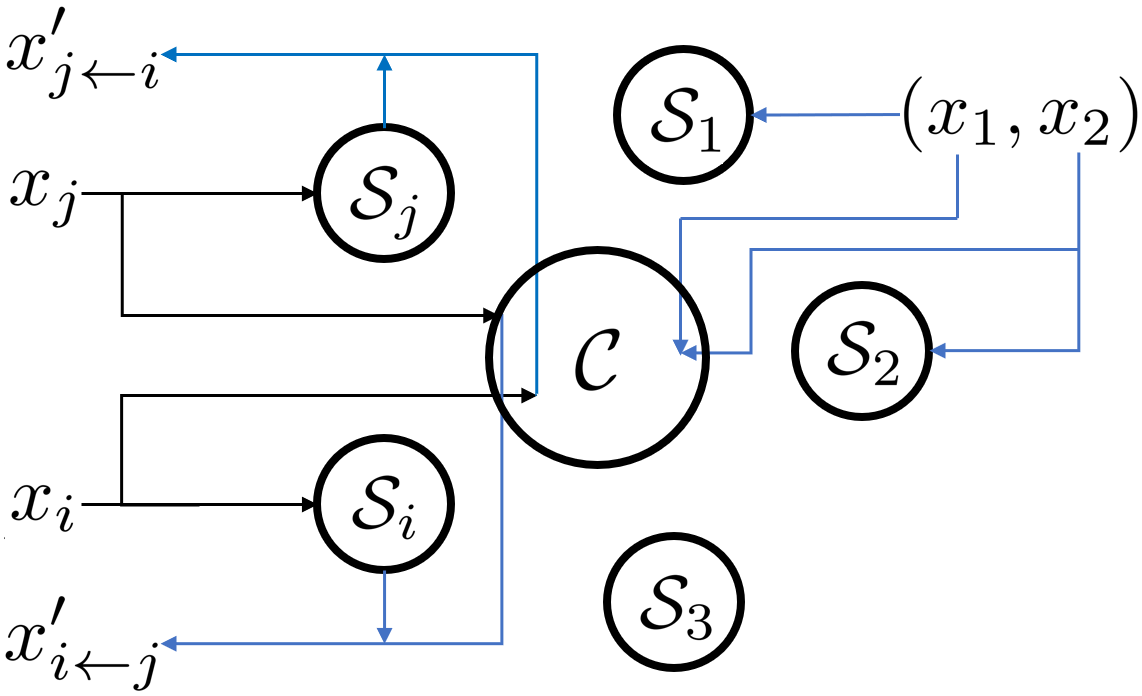
\includegraphics[width=0.55\textwidth]{FIG/model}
\caption{Autoencoder model with partially shared latent space. Sample $x_i$ is encoded into a domain-specific space $\mathcal{S}_i$ and a shared content space $\mathcal{C}$. Corresponding datapoints $(x_1,x_2)$ are encoded in the same content code. Converted sample $x_{j\leftarrow i}'$ is generated by recombining the original content code of $x_i$ and the style code randomly sampled from $\mathcal{S}_j$.}
\label{fig:model}
\end{figure}

We formulate the learning problem as a distributionally robust game. Each domain $i$ has four agents $E_i^c, E_i^s, G_i, D_i$, in which $D_i$ is a discriminator with two objectives. One is to distinguish between real samples and machine-generated samples, the other is to classify domain labels. On the other side, the generators $G_i$ have two purposes: synthesize realistic samples and convert them into domain $i$. For example in voice conversion, the synthesized speech is evaluated on both the naturalness of its quality and the correctness of speaker's identity.


\subsubsection{Two-domain transformation}
There are $4n$ agents for $n$ domains. For simplicity, we first investigate the conversion model between two domains. When $n=2$, there are 8 agents: $E^c_1, E^s_1, G_1, D_1$ for domain $\mathbb{X}_1$ and $E^c_2, E^s_2, G_2, D_2$ for domain $\mathbb{X}_2$. Each agent has a different objective, and the utility function of one agent depends on the action of other agents. Collaboration and competition exist among them. So this is a distributionally robust game with cooperative agents and uncertain utility functions.
Based on the analysis above, there are five modules need to learn:
\begin{enumerate}
\item [\circled{1}] domain-invariant content encoder
\item [\circled{2}] domain-specific style encoders
\item [\circled{3}] real/fake discriminator
\item [\circled{4}] domain classifier $D_i$
\item [\circled{5}] fake samples generator
\end{enumerate}

The encoders and decoders form a group to synthesize converted samples in the target domain. Another group is the discriminator and classifier. They work on the opposite side to distinguish between real/fake samples and predict the domain label. The intergroup competition and intragroup collaboration are listed in table \ref{tab:game}.

{\color{blue} How to define the game? \\
When Nash equilibrium reaches, the autoencoder $(E^{c*}_i, E^{s*}_i, G^*_i)$ minimizes the reconstruction error $L^x_{rec}\rightarrow0, L^c_{rec}\rightarrow0, L^s_{rec}\rightarrow0$. The GAN network $(D^*_i, G^*_i)$ and adversarial loss $L^{x_i}_{GAN}$ converge at saddle points that minimize the distance between $p(x_i)$ and $p(x_{j\leftarrow i}')$. The classifier $D^{cls*}_i$ correctly predicts the domain category of both real and fake samples $D^{cls*}_i(x_i)=i$, $D^{cls*}_i(x_{i\leftarrow j}')=i$.
}

\begin{table}[htb]
\centering
\caption{Cooperative game}
%\resizebox{0.5\textwidth}{!}{%
\begin{tabular}{|c|c|c|}
\hline
Intergroup competition   & Learning module & Objective          \\ \hline
$E^s_1, E^s_2$      & \circled{2}       & $\min L^s_{cyc}$      \\ \hline
$D_1, D_2$          & \circled{4}       & $\min L^x_{cls}$      \\ \hline
\hline
Intragroup collaboration & Learning module & Objective          \\ \hline
$E^c_1, E^s_1, G_1$ & $Autoencoder_1$   & $\min L^{x_1}_{rec}$  \\ \hline
$E^c_2, E^s_2, G_2$ & $Autoencoder_2$   & $\min L^{x_2}_{rec}$  \\ \hline
$G_1, G_2$          & \circled{5}       & $\min L^x_{GAN}$      \\ \hline
$D_1, D_2$          & \circled{3}       & $\max L^x_{GAN}$      \\ \hline
$E_1^c, E_2^c$      & \circled{1}       & $\min L^c_{cyc}$      \\ \hline

\end{tabular}%}
\label{tab:game}
\end{table}

{\color{blue}
The collaboration means, agents in different domains can help each other as they may have common interests. For instance, a sample can be used to update the real/fake discriminator even if its class label is missing. Except for the autoencoders $E^c_i, E^s_i, G_i$, other coalitions are cross-domain. $(G_1, G_2)$ works on data synthesis, $D_1, D_2$ works on real/fake discrimination, $E^c_1, E^c_2$ extracts high-level content information that we want to preserve.
}

We jointly train the encoders, decoders and GAN's discriminators with multiple objectives. To keep encoder and decoder as inverse operations, a reconstruction loss is applied in the direction $x_i \rightarrow (c_i, s_i) \rightarrow x_i'$, ($i,j \in {1,2}$). Sample $x_i$ should not be changed after encoding and decoding.
\begin{equation}
L_{rec}^{x_i} = \mathbb{E}_{x_i}(\| x_i - x_i' \|_1), \quad x_i' = G_i(E_i^c(x_i), E_i^s(x_i))
\end{equation}

%\begin{figure}[htb]
%\centering
%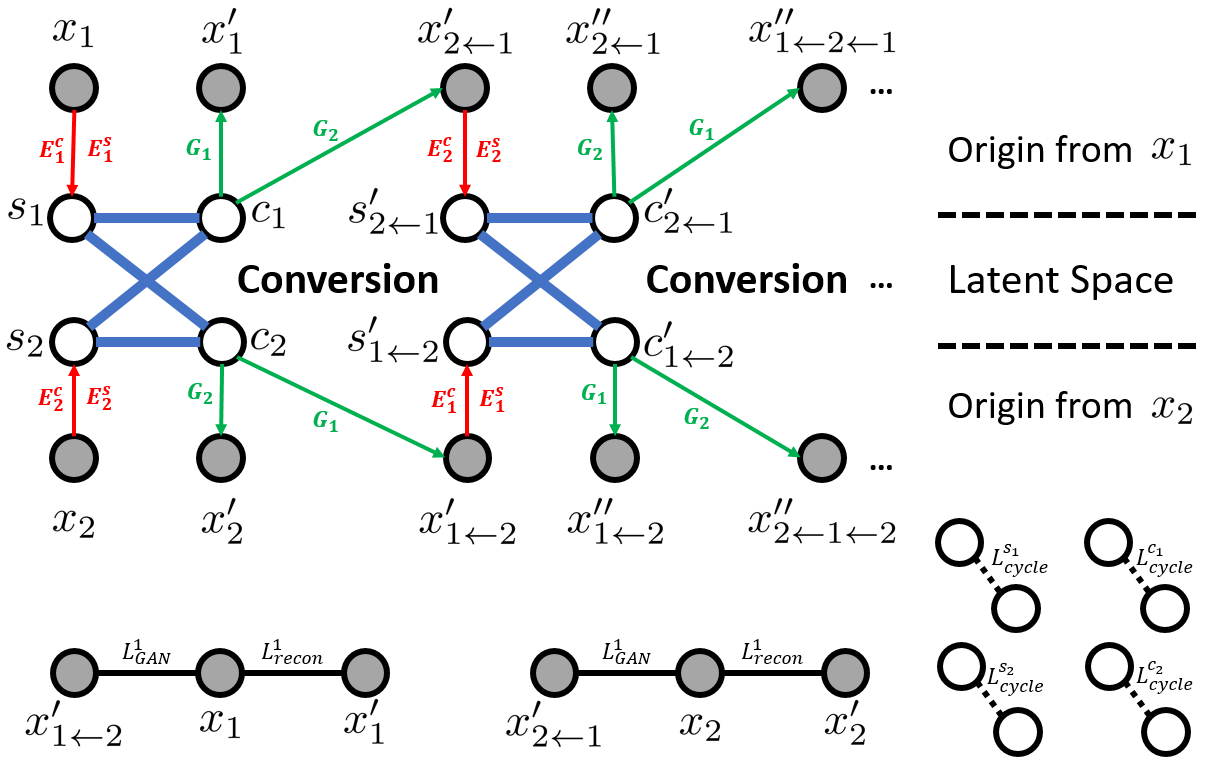
\includegraphics[width=0.7\textwidth]{FIG/loss}
%\caption{Train on multiple objectives}
%\label{loss}
%\end{figure}

In our model, the latent space is partially shared. Thus the cycle consistency constraint [10] is not preserved, i.e., $x_{1\leftarrow2\leftarrow1}'' \neq x_1$. We apply a semi-cycle loss in the coding direction $c_1 \rightarrow x_{2\leftarrow1}' \rightarrow c_{2\leftarrow1}'$ and $s_2 \rightarrow x_{2\leftarrow1}' \rightarrow s_{2\leftarrow1}'$.
\begin{equation}
\begin{aligned}
L_{cyc}^{c_1} = \mathbb{E}_{c_1, s_2} (\| c_1 - c_{2\leftarrow1}' \|_1), \quad c_{2\leftarrow1}'=E_2^c(x_{2\leftarrow1}') \\
L_{cyc}^{s_2} = \mathbb{E}_{c_1, s_2} (\| s_2 - s_{2\leftarrow1}' \|_1), \quad s_{2\leftarrow1}'=E_2^s(x_{2\leftarrow1}')
\end{aligned}
\end{equation}
Moreover, we add a GAN module to ensure the quality of generated samples. They should be indistinguishable from the real samples in the target domain $\mathbb{X}_i$. GAN loss is computed between $x_j$ and $x_{i\leftarrow j}'$ to represent the distance between two distributions $p(x_j)$, $p(x_{i\leftarrow j}')$.
\begin{equation}
L_{GAN}^{x_i} = \mathbb{E}_{c_j, s_i}[\log(1-D_i(x_{i\leftarrow j}'))] + \mathbb{E}_{x_i}[\log D_i(x_i)]
\end{equation}
The full loss is the weighted sum of $L_{recon}$, $L_{cycle}$, $L_{GAN}$.
\begin{equation}
\begin{aligned}
&\min_{E_1^c,E_1^s,E_2^c,E_2^s, G_1,G_2}\max_{D_1,D_2} L(E_1^c, E_1^s, E_2^c, E_2^s, G_1, G_2, D_1, D_2) \\
&= \lambda_s (L_{cyc}^{s_1} + L_{cyc}^{s_2}) + \lambda_c (L_{cyc}^{c_1} + L_{cyc}^{c_2}) + \lambda_x (L_{rec}^{x_1} + L_{rec}^{x_2}) + \lambda_g (L_{GAN}^{x_1} + L_{GAN}^{x_2})
\end{aligned}
\end{equation}
where $\lambda_s, \lambda_c, \lambda_x, \lambda_g$ control the weights of the components.
% $L^x_{cls}$ is the KL divergence between two classes.


\subsubsection{Multi-domain transformation}
In multi-domain case, there are $4n$ agents in the game. To reduce complexity, we replace the domain-specific models $E^c_i, G_i, D_i$ with a shared content encoder $E^c$, a shared decoder $G$, and a single multiclass classifier $D^{cls}$. Thus, only $n+3$ agents left. {\color{blue} (form coalition?)} Figure \ref{fig:multi} shows the multi-domain transformation model.

\begin{figure}[htb]
\center
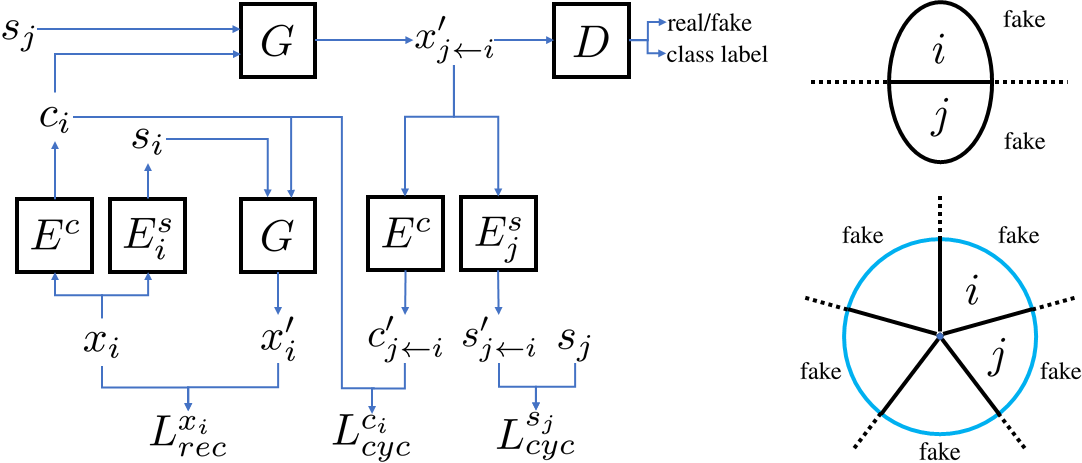
\includegraphics[width=0.8\textwidth]{FIG/multi}
\caption{Learn multi-domain transformation. Left: conversion model with shared content encoder, decoder and classifier. Top-right: two domains. Bottom-right: multiple domains (n=5).}
\label{fig:multi}
\end{figure}

When $n=2$, there are 3 kinds of data: real in $\mathbb{X}_1$, real in $\mathbb{X}_2$ and fake in $\mathbb{X}_{fake}$. Two real/fake discriminators $D_1,D_2$ are enough for classification.
%, so $D^{cls}$ is ommitted.
If this idea is extended to multiple domains, there will be $n$ binary discriminators and $2^n$ outputs. Instead, we replace them with one binary real/fake discriminator $D$ and one multiclass domain classifier $D^{cls}$. The two-step classification not only reduces complexity ($2n$ outputs) but also makes the most of the training data. An example in domain $i$ is also useful to train the generative model for other domains, as it is the common interest of all agents $G_1, G_2, \ldots G_n$ to synthesize realistic data. Therefore, the multi-domain transformation model can be trained on different datasets with partially labeled data.

In the following sections, we will apply the proposed method on two real-world applications: image style transfer and emotinal speech conversion.


\subsection{Case Study: Image Style Transfer}
Image style transfer, or image-to-image translation is a hot topic in computer vision. The objective is to transfer the visual style of an image while keep its semantic content. Similar tasks includes texture synthesis, artistic style transfer, photorealistic image style transfer, etc.

Gatys et al. [7] introduced an algorithm to separate and recombine the content and style of natural images. They claimed that a Convolutional Neural Network (CNN) is the ideal representation to factorize semantic content and artistic style. High-level features are extracted by higher layers of the network, while low-level features are captured by the correlations between filter responses in various layers. However, the style is learnt from a single image, which limits the ability to capture the general theme of the target domain.
%It can preserve the semantic content of source image and replace the style with that learnt from the target image.

Instead of example-based style transfer, we will focus on leanring the translation model between two image distributions. There are a broad range of researches on image synthesis and representation learning. We will expore the state-of-the-art neural network architecture and implement our model to learn the disentangled representations of image style and content. The proposed method will be tested on a typical image style transfer task.


\subsection{Case Study: Emotional Voice Conversion}
Voice transformation (VT) is a technique to modify some properties of human speech while preserving its linguistic information. VT can be applied to change the speaker identity, i.e., voice conversion (VC) [50], or to transform the speaking style of a speaker, such as emotion and accent conversion [65]. In this section, we will focus on emotion voice transformation. The goal is to change emotion-related characteristics of a speech signal while preserving its linguistic content and speaker identity. Emotion conversion techniques can be applied to various tasks, such as hiding negative emotions for customer service agents, helping film dubbing, and creating more expressive voice messages on social media.

Existing VC approaches cannot be applied directly because they change speaker identity by assuming pronunciation and intonation to be a part of the speaker-independent information. Since the speaker's emotion is mainly conveyed by prosodic aspects, some studies have focused on modelling prosodic features such as pitch, tempo, and volume [66][67]. In [68], a rule-based emotional voice conversion system was proposed. It modifies prosody-related acoustic features of neutral speech to generate different types of emotions. A speech analysis-synthesis tool STRAIGHT [52] was used to extract fundamental frequency ($F_0$) and power envelope from raw audio. These features were parameterized and modified based on Fujisaki model [69] and target prediction model [70]. The converted features were then fed back into STRAIGHT to re-synthesize speech waveforms with desired emotions. However, this method requires temporal aligned parallel data that is difficult to obtain in real applications; and the accurate time alignment needs manual segmentation of the speech signal at phoneme level, which is very time consuming.

To address these issues, we propose a nonparallel training method. Instead of learning example based one-to-one mapping between paired emotional utterances $(x_1, x_2)$, we learn the conversion model between two emotion domains $(\mathbb{X}_1, \mathbb{X}_2)$.

Inspired by the disentangled representation learning in image style transfer [31][9], we assume that each speech signal $x_i \in \mathbb{X}_i$ can be decomposed into a content code $c \in \mathcal{C}$ that represents emotion-invariant information and a style code $s_i \in \mathcal{S}_i$ that represents emotion-dependent information. $\mathcal{C}$ is shared across domains and contains the information we want to preserve. $\mathcal{S}_i$ is domain-specific and contains the information we want to change. In conversion stage, we extract content code of the source speech and recombine it with style code of the target emotion. A generative adversarial network (GAN) [15] is added to improve the quality of converted speech. Our approach is nonparallel, text-independent, and does not rely on any manual operation.

For implementation, we use deep neural networks to learn the latent representations of speech. Specifically, the encoders and decoders are implemented with one-dimensional CNNs to capture the temporal dependences. The GAN discriminators are implemented with two-dimensional CNNs to capture the spectra-temporal patterns. All networks are equipped with gated linear units (GLU) [73] as activation functions.

We plan to test our approach on IEMOCAP [71] to learn the conversion models for four emotions: angry, happy, neutral, sad. IEMOCAP is a nonparallel dataset widely used in emotional speech recognition and analysis. It contains scripted and improvised dialogs in five sessions; each has labeled emotional sentences pronounced by two professional English speakers. The emotions in scripted dialogs have strong correlation with the lingual content. Since our task is to change emotion but keep the speaker identity and linguistic content, we only use the improvised dialogs of the same speaker.

There are three metrics for performance evaluation: emotion correctness, voice quality and the ability to retain speaker identity. For subjective evaluation, we will conduct listening tests on Amazon MTurk to evaluate the converted speech. Each example is evaluated by a group of random listeners. They will be asked to manually classify the emotion, and give 1-to-5 opinion scores on voice quality and the similarity with the original speaker. The classification result and mean opinion score (MOS) are two major measurements. For objective evaluation, we plan to use the state-of-the-art speech emotion classifier [72] to check the emotion category of generated speech. It indicates a success if our model can increase the proportion of the target emotions and reduce the original emotions.  To our knowledge, this is the first work for nonparallel emotion conversion. If there's time, we will develop multidomain emotion conversion models for unseen speakers.


%(animal voice conversion -- cat/dog voice recognition)

%$\mathcal{S}_i, \mathcal{S}_j, \mathcal{S}_1, \mathcal{S}_2, \mathcal{S}_3$
%$c_i, s_i, s_j, x_i, x_i', c_{j\leftarrow i}', s_{j\leftarrow i}'$
%$L^{x_i}_{rec}, L^{c_i}_{cyc}, L^{s_j}_{cyc}$
%$E^c, E^s_i, E^s_j, G, D, i, j$
%fake, class label, real



\newpage



\section{Dissertation Outline}
\label{Sec:Outline}

The research will be split into the following four stages:

\subsection{Introduction}

\subsection{Related Work}

\subsection{Distributionally Robust Games}
%Problem Formulation
In this part we introduce distributionally robust games and develop new filtering and learning architectures under this framework. The system may contain several competing neural networks: the attackers learn to generate synthetic samples that are supposed to have the same distribution as the original ones, while the defenders try to find counter-examples and create difficulties for the other side. Each player tries to perform better and beat the others, which forms a multi-agent zero-sum game with uncertain payoffs. The players use a robust optimization approach to contend with the worst-case scenario payoff. The attacker network is constructed based on the outcome of defender networks, and vice versa. The competing networks are trained together iteratively until achieving the distributional robust Nash equilibrium.

\subsection{Wasserstein Metric}
The loss function is designed to measure the similarity of two probability distributions. Unsupervised learning is conducted by minimizing the loss. We plan to study the properties of several widely used loss metrics:
\begin{itemize}
\item Compare L1, L2-loss, KL-divergence, f-divergence, and Wasserstein distance
\item Study the time-dependent formulation of the optimal transportation cost
\item Test the effect of translation and perturbation for a certain loss metric
\end{itemize}

\subsection{Learning Algorithms for Robust Optimization}
\begin{itemize}
\item Develop a specific learning algorithm to find robust Nash equilibria, which should be stable and efficient
\item Compare with existing numerical optimization approaches in large-scale machine learning: SGD, Adam, Momentum, Ishikawa-Nesterov, Newton's method, conjugate gradient, natural gradient, etc.
\item Compare with existing deep generative models: RBM, VAE, GAN, WGAN, etc.
\end{itemize}

\subsection{Generative Modeling for Vehicle Tracking}
\subsection{Generative Modeling for Image Synthesis}
\subsection{Generative Modeling for Voice Conversion}

\subsection{Experiments on Large-scale Machine Learning datasets}
\begin{itemize}
\item Maryland Traffic Surveillance Dataset (Vehicle tracking)
\item Large-scale CelebFaces Attributes Dataset (CelebA, image synthesis)
\item Large-scale Scene Understanding Challenge (LSUN, image synthesis)
\item Interactive Emotional Dyadic Motion Capture (IEMOCAP, emotional voice conversion)
\end{itemize}

\subsection{Discussion}

\subsection{Conclusion and Future Work}



\section{Research Plan}
\label{Sec:Plan}

\subsection{Research Progress}
\begin{itemize}
\item[] Literature review, planning
\item[] Theory part on distributional robust games, Bregman learning and convex optimization
\item[] Theoretical analysis and comparison for L2 distance, f-divergence and Wasserstein metric
\item[] Algorithm design, overall integration, simulations, specific implementations on real problems
\item[] Application part on large-scale machine learning: experiments, evaluation and revision
\item[] Documentation and Defence
\end{itemize}

\subsection{Application on Image and Audio Synthesis}
\begin{itemize}
\item Test on large-scale image dataset MNIST, CelebA and LSUN
\item Literature review on emotional speech classification and audio synthesis
\item Compare two sound representations in generative learning: waveform and spectrogram
\item Design deep generative models for emotional speech generation
\item Test on voice conversion or music style transfer if possible
\end{itemize}


\subsection{Timeline}
\begin{align*}
&\text{Fall 2018} && \text{Study on Generative Models for Voice Conversion} \\
&\text{Spring 2019} && \text{Write Thesis} \\
&\text{August 2019} && \text{Thesis Defense}
\end{align*}


%\subsection{Long-term, from Feb 2018}
%\subsection{Short-term, from Spet 2018 (need discussion)}
%Week 1-2: Literature review on deep generative models, sound classification and audio synthesis \\
%Week 3-4: Investigation on two audio synthesis tasks: emotional speech generation and music style transfer \\
%Week 5-6: Compare two sound representations in generative learning: waveform and spectrogram \\
%Week 7-8: Algorithm design and experiments; submit a paper to ICASSP if possible \\
%Week 9-12: Refine the model, test on voice conversion and music style transfer if possible.



\section{Conclusion}
\label{Sec:Con}

Tackling the aforementioned problems would take us much closer to
real intelligent systems, and defines three core pillars
of Artificial Intelligence. However, there are many other problems which
need to be solved and integrated to achieve a fully
intelligent system, e.g. navigation, learning by imitation, cooperation, and many others.

%However, I think that all that skills can be integrated by means of external interface, and
%don't have to be modeled in any special way. For instance, navigation skill could emerge
%as an use two interfaces (1) GPS location interface, and (2) an external memory.

%This is my personal opinion, and it shouldn't be judged in a scientific way.
%I strongly believe that creation of artificial intelligence is potentially
%dangerous. However, I think, that more dangerous is avoiding to create it.
%We exhaust resources of our planet in rapid fashion, and lack of resources
%leads to wars. The only way to prevent it is to have abundance of resources.
%Artificial intelligence could provide abundance of all resources.



\section{List of Publications}
\label{Sec:Pub}

\subsection{Thesis Related Publications}
\begin{enumerate}
\item[] Jian Gao and Hamidou Tembine, Distributionally Robust Games for Deep Generative Learning, July 2018. DOI: 10.13140/RG.2.2.15305.44644
\item[] Jian Gao, Yida Xu, Julian Barreiro-Gomez, Massa Ndong, Michalis Smyrnakis and Hamidou Tembine (September 5th 2018) \href{https://www.intechopen.com/books/optimization-algorithms-examples/distributionally-robust-optimization}{Distributionally Robust Optimization}. In Jan Valdman, Optimization Algorithms, IntechOpen. DOI: 10.5772/intechopen.76686. ISBN: 978-1-78923-677-4
\item[] Jian Gao and Hamidou Tembine, Distributionally Robust Games: Wasserstein Metric, International Joint Conference on Neural Networks (IJCNN), Rio de Janeiro, Brazil, July 2018
\item[] Jian Gao and Hamidou Tembine, Bregman Learning for Generative Adversarial Networks, Chinese Control and Decision Conference (CCDC), Shenyang, China, June 2018 \textit{(Best Paper Finalist Award)}
\item[] Jian Gao and Hamidou Tembine, Distributed Mean-Field-Type Filter for Vehicle Tracking, in American Control Conference (ACC), Seattle, USA, May 2017 \textit{(Student Travel Award)}
\item[] Dario Bauso, Jian Gao and Hamidou Tembine, Distributionally Robust Games: f-Divergence and Learning, 11th EAI International Conference on Performance Evaluation Methodologies and Tools (VALUETOOLS), Venice, Italy, Dec 2017
%    \item Jian Gao and Hamidou Tembine, A mean-field filter for two-step ahead forward-looking problems, Workshop on Frontiers of Networks: Theory and Algorithms , Seventeenth International Symposium on Mobile Ad Hoc Networking and Computing, MobiHoc, July 5-7,2016, Paderborn, Germany
\end{enumerate}


\subsection{Other Publications}
\begin{enumerate}
\item[] J. Gao and H. Tembine, "Distributed Mean-Field-Type Filters for Traffic Networks," in IEEE Transactions on Intelligent Transportation Systems. doi: 10.1109/TITS.2018.2816811
\item[] J. Gao and H. Tembine, "Empathy and berge equilibria in the forwarding dilemma in relay-enabled networks," 2017 International Conference on Wireless Networks and Mobile Communications (WINCOM), Rabat, 2017, pp. 1-8. doi: 10.1109/WINCOM.2017.8238199 \href{https://nyuad.nyu.edu/en/news/latest-news/science-and-technology/2017/december/next-generation-cell-phone-networks.html}{(\textit{Best paper Award})}
\item[] J. Gao and H. Tembine, "Correlative mean-field filter for sequential and spatial data processing," IEEE EUROCON 2017 -17th International Conference on Smart Technologies, Ohrid, 2017, pp. 243-248. doi: 10.1109/EUROCON.2017.8011113
\item[] Fanhuai Shi, Jian Gao, Xixia Huang, An affine invariant approach for dense wide baseline image matching. International Journal of Distributed Sensor Networks (IJDSN) 12(12) (2016)
\item[] J. Gao and H. Tembine, "Distributed Mean-Field-Type Filters for Big Data Assimilation," 2016 IEEE 18th International Conference on High Performance Computing and Communications; IEEE 14th International Conference on Smart City; IEEE 2nd International Conference on Data Science and Systems (HPCC/SmartCity/DSS), Sydney, NSW, 2016, pp. 1446-1453. doi: 10.1109/HPCC-SmartCity-DSS.2016.0206
\end{enumerate}



%\subsubsection*{Acknowledgments}
%
%Use unnumbered third level headings for the acknowledgments. All
%acknowledgments go at the end of the paper. Do not include
%acknowledgments in the anonymized submission, only in the final paper.

\cite{NIPS2014_5423}



%\section*{References}

%References follow the acknowledgments. Use unnumbered first-level
%heading for the references. Any choice of citation style is acceptable
%as long as you are consistent. It is permissible to reduce the font
%size to \verb+small+ (9 point) when listing the references. {\bf
%  Remember that you can use more than eight pages as long as the
%  additional pages contain \emph{only} cited references.}
%
%\medskip
%
%\small
%
%[1] Alexander, J.A.\ \& Mozer, M.C.\ (1995) Template-based algorithms
%for connectionist rule extraction. In G.\ Tesauro, D.S.\ Touretzky and
%T.K.\ Leen (eds.), {\it Advances in Neural Information Processing
%  Systems 7}, pp.\ 609--616. Cambridge, MA: MIT Press.
%
%[2] Bower, J.M.\ \& Beeman, D.\ (1995) {\it The Book of GENESIS:
%  Exploring Realistic Neural Models with the GEneral NEural SImulation
%  System.}  New York: TELOS/Springer--Verlag.
%
%[3] Hasselmo, M.E., Schnell, E.\ \& Barkai, E.\ (1995) Dynamics of
%learning and recall at excitatory recurrent synapses and cholinergic
%modulation in rat hippocampal region CA3. {\it Journal of
%  Neuroscience} {\bf 15}(7):5249-5262.



\bibliographystyle{unsrt}
\bibliography{ref}



\end{document}



%[1] T. Lindvall, Lectures on the coupling method. Wiley, New York, 1992.
%[2] Unsupervised pixel-level domain adaptation with generative adversarial networks
%[3] Learning from simulated and unsupervised images through adversarial training
%[4] Unsupervised cross-domain image generation.
%[5] Improving predictive inference under covariate shift by weighting the log-likelihood function
%[6] Direct Importance Estimation with Model Selection and Its Application to Covariate Shift Adaptation
%[7] Image Style Transfer Using Convolutional Neural Networks
%[8] Unsupervised image-to-image translation networks
%[9] Multimodal Unsupervised Image-to-Image Translation
%[10] Unpaired image-to-image translation using cycle-consistent adversarial networks (CycleGAN)
%[11] Domain adaptation with conditional transferable components
%[12] Bregman divergence-based regularization for transfer subspace learning
%[13] Domain-adversarial training of neural networks
%[14] DeepJDOT: Deep Joint Distribution Optimal Transport for Unsupervised Domain Adaptation
%[15] Generative Adversarial Nets
%[16] Auto-Encoding Variational Bayes
%[17] Pixel Recurrent Neural Networks
%[18] DCGAN
%[19] Progressive growing of GANs for improved Quality, Stability, and Variation
%[20] Conditional Generative Adversarial Nets
%[21] Deep Generative Image Models using a Laplacian Pyramid of Adversarial Networks
%[22] Improved Training of Wasserstein GANs
%[23] Autoencoding beyond pixels using a learned similarity metric
%[24] WAVENET: A GENERATIVE MODEL FOR RAW AUDIO
%[25] Pixel Recurrent Neural Networks
%[26] Conditional Image Generation with PixelCNN Decoders
%[27] State of the "Art": A Taxonomy of Artistic Stylization Techniques for Images and Video
%[28] Style-transfer via texture-synthesis.
%[29] Generative Visual Manipulation on the Natural Image Manifold
%[30] A Closed-form Solution to Photorealistic Image Stylization
%[31] Image Style Transfer Using Convolutional Neural Networks
%[32] A Neural Algorithm of Artistic Style
%[33] Image-to-image translation with conditional adversarial networks
%[34] Unsupervised crossdomain image generation.
%[35] Generative attribute controller with conditional filtered generative adversarial networks
%[36] Universal Style Transfer via Feature Transforms
%[37] High-Resolution Image Synthesis and Semantic Manipulation with Conditional GANs
%[38] Learning to generate images of outdoor scenes from attributes and semantic layouts
%[39] Photo-realistic single image superresolution using a generative adversarial network.
%[40] Colorful image colorization.
%[41] Age progression/regression by conditional adversarial autoencoder.
%[42] Perceptual losses for real-time style transfer and super-resolution.
%[43] Generative image modeling using style and structure adversarial networks.
%[44] Coupled generative adversarial networks (CoGAN)
%[45] Domain-Adversarial Training of Neural Networks (DANN)
%[46] Learning transferable features with deep adaptation networks (DAN)
%[47] Deep Hashing Network for Unsupervised Domain Adaptation
%[48] Optimal transport for domain adaptation
%[49] Joint distribution optimal transportation for domain adaptation
%[50] An overview of voice conversion systems
%[51] The Voice Conversion Challenge 2018: Promoting Development of Parallel and Nonparallel Methods
%[52] Restructuring speech representations using a pitchadaptive time-frequency smoothing and an instantaneousfrequency-based f0 extraction: possible role of a repetitive structure in sounds (STRAIGHT)
%[53] Speaker-dependent WaveNet vocoder
%[54] Improved HNM-based Vocoder for Statistical Synthesizers
%[55] High-Order Sequence Modeling Using Speaker-Dependent Recurrent Temporal Restricted Boltzmann Machines for Voice Conversion
%[56] Voice conversion through vector quantization
%[57] Continuous Probabilistic Transform For Voice Conversion
%[58] Exemplarbased sparse representation with residual compensation for voice conversion
%[59] Signal estimation from modified short-time Fourier transform
%[60] Text-independent voice conversion based on unit selection
%[61] A KL divergence and DNN-based approach to voice conversion without parallel training sentences
%[62] Voice conversion from unaligned corpora using variational autoencoding Wasserstein generative adversarial network
%[63] Phonetic posteriorgrams for many-to-one voice conversion without parallel data training
%[64] PARALLEL-DATA-FREE VOICE CONVERSION USING CYCLE-CONSISTENT ADVERSARIAL NETWORKS
%[65] Accent conversion using phonetic posteriorgrams
%[66] Emotional voice conversion for mandarin using tone nucleus model–small corpus and high efficiency
%[67] Multi-level prosody and spectrum conversion for emotional speech synthesis
%[68] Voice conversion for emotional speech: Rule-based synthesis with degree of emotion controllable in dimensional space
%[69] Analysis of voice fundamental frequency contours for declarative sentences of japanese
%[70] A study on applying target prediction model to parameterize power envelope of emotional speech
%[71] Iemocap: Interactive emotional dyadic motion capture database
%[72] Automatic speech emotion recognition using recurrent neural networks with local attention
%[73] Language modeling with gated convolutional networks
%[74] Large Scale GAN Training for High Fidelity Natural Image Synthesis
%[75] MuseGAN: Multi-Track Sequential Generative Adversarial Networks for Symbolic Music Generation and Accompaniment
%[76] StarGAN: Unified Generative Adversarial Networks for Multi-Domain Image-to-Image Translation
%[77] Generating Text through Adversarial Training using Skip-Thought Vectors
%[78] A Universal Music Translation Network
%[79] ImageNet: A Large-Scale Hierarchical Image Database
